\chapter{Обработка информации с прибора} \label{chapt3}


Отладка программного обеспечения и проверка обработки сигналов от детекторов на этапе  конструкторских работ производилась подключением канала RS232 к последовательному (COM) порту персонального компьютера. Программное обеспечение контроллера формирует отладочные посылки и массивы тестовых данных и отправляет по интерфейсу USART, реализованному на всех использовавшихся контроллерах. Такой способ передачи тестовых данных выбран как максимально приближенный к условиям реального функционирования прибора. 

Автономные испытания Дэпрон проходили с момента создания первых версий ПМО до ноября 2011. В ходе этих испытаний были проведены основные калибровки усилительных трактов прибора с помошью генератора сигналов и с помошью  источников ионизирующего излучения.

Отработка работы прибора в комплексе научной аппаратуры позволяет использовать штатный способ передачи информации по каналу CAN, в таком случае критерием работы прибора является выдача от БИ содержательных блоков информации с меткой, соответствующей прибору ДЭПРОН. 

\section{Схема обработки информации при КДИ}\label{sec3.1}

Для обработки данных и отладки работы прибора ДЭПРОН были использованы специально разработанные программные средства. Поскольку отладка прибора ДЭПРОН производится подключением по каналу RS232 а при работе в штатном режиме передача данных ведется по каналу CAN, для взаимодействия с прибором были написаны две различные программы.

\subsection{Отладочная программа Depron Terminal}

Данная программа предназначена для отладки прибора во время лабораторных испытаний, проверки работоспособности прибора при приемо-сдаточных работах. Программа была написана в средстве разработки ПО Microsoft Visual Studio на языке C\#, c использованием фрэймворка .NET3.5. Пользовательский интерфейс программы построен на основе WinForms, поэтому отличается консервативностью и достаточно низкими аппаратными требованиями.

Программа позволяет:


\begin{itemize}
	\item 	Подключаться к прибору ДЭПРОН по каналу RS232 (с использованием COM порта)
	
	
	\item 	Принимать и отображать тестовые данные сформированные прибором ДЭПРОН
	
	
	\item 	Сохранять запись потока данных на жесткий диск ПК (в фоновом режиме и по запросу)
	
	
	\item 	Открывать сохраненные данные с носителя информации
	
	
	\item 	Посылать команды на прибор ДЭПРОН (в том числе с заданной периодичностью)
	
	
\end{itemize}
\begin{figure}
\centering
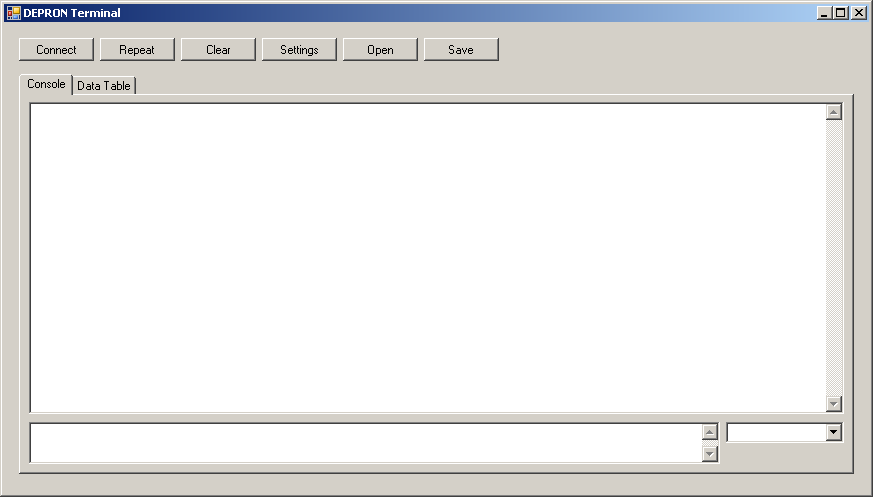
\includegraphics[width=0.7\linewidth]{images/depron_terminal}
\caption{Интерфейс программы \textbf{Depron Terminal}}
\label{fig:depron_terminal}
\end{figure}

Данная программа была использована как основа для разработки отладочной программы для дозиметрических блоков ДБ-8м. Основные принципы работы новой программы, названной \textbf{DB8m Terminal} были сохранены и она обеспечивает те же базовые функции. Дополнительно программа обеспечивает возможность накопления спектров энерговыделения по детекторам ДБ-8м и отображения их в графическом виде, в режиме реального времени. 
\begin{figure}
\centering
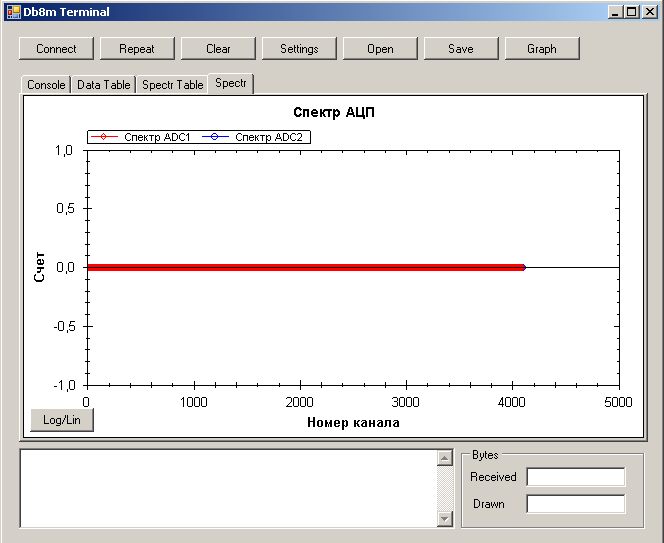
\includegraphics[width=0.7\linewidth]{images/db8m_terminal}
\caption{Интерфейс программы \textbf{DB8mTerminal}}
\label{fig:db8m_terminal}
\end{figure}

Графическое отображение спектров реализовано с использованием компонента ZedGraph. Введение такой возможности значительно ускорило калибровку и градуировку прибора на источниках радиационного излучения, так что может быть рекомендовано для программ аналогичной направленности.

\subsection{Программа DepronExplorerView}

Данная программа предназначена для просмотра и обработки данных прибора полученных во время комплексных испытаний или во время штатной работы прибора. Аналогично Depron Terminal, данная программа была написана в средстве разработки ПО Microsoft Visual Studio на языке c\# c использованием фрэймворка .NET3.5. Пользовательский интерфейс программы построен на основе WPF.


На момент комплексных испытаний прибора ДЭПРОН программа DepronExplorerView позволяет отображать все типы бинарных данных, полученных от прибора ДЭПРОН, в таблично-текстовой форме и сохранять полученные данные в текстовые файлы. Для удобства использования интерфейс программы выполнен в стиле файлового менеджера. 

Подготовленная программа активно использовлалась при всех испытаниях прибора ДЭПРОН в комплексе аппаратуры спутника, а также будет использоваться при предполетных проверках на космодроме Восточный.

\begin{figure}
\centering
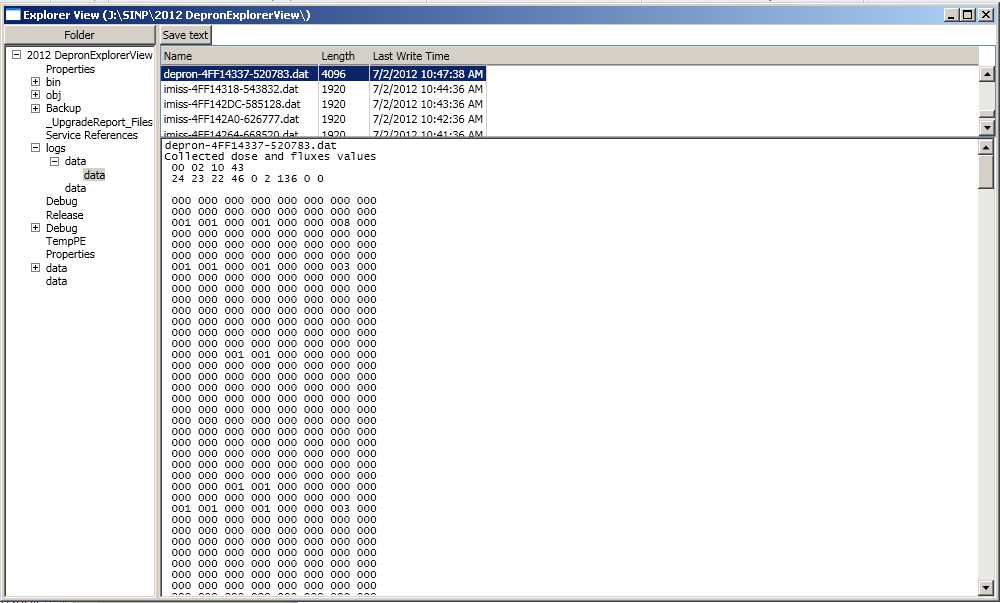
\includegraphics[width=0.8\linewidth]{images/depron_explorer}
\caption{Интерфейс программы \textbf{DepronExplorerView}}
\label{fig:depron_explorer}
\end{figure}


\subsection{Структура массивов (базы данных) результатов измерений}

Результаты измерений прибора ДЭПРОН формируется в массивы информации размером 512 байт.


Каждое сообщение состоит из следующих полей:

\begin{itemize}
	\item  начало сообщения;

	\item  категория;

	\item  длина сообщения;

	\item  данные.
\end{itemize}


Поле {``}начало сообщения'' содержит 2 байта:
\begin{itemize}
	\item байт DLE -- 11110000;
	\item байт STX -- 11111111.
\end{itemize}


На момент написания в программе ДЭПРОН используются нестандартные значения для байт DLE и STX, поэтому во избежание путаницы в дальнейших версия ПО ДЭПРОН будут использоваться общепринятые значения этих байт.


Поле ``категория'' состоит из одного байта (CAT). При обмене с БИ используются варианты сообщений: A, S, H, N. Коды сообщений соответствуют таблице ASCII: A - 01000001, S - 01010011, H - 01001000, N -- 01001110.

Поле ``длина сообщения'' содержит 1 байт (LEN) по умолчанию передается ``\ensuremath{\backslash 0}'', что означает общую длину посылки 512 байт.


В ином случае значение длины равно общему числу байт сообщения, исключая поле ``начало сообщения''.


Поле ``данные'' (RECORD) содержит данные в соответствии с описанием передаваемых сообщений и их спецификацией.



Общая структура сообщений выглядит следующим образом:

\begin{tabular}{|p{4.5cm}|c|c|p{2.5cm}|}
	\hline
	Начало сообщения (DLE,STX) & Категория(CAT) & Длина(LEN)  & Данные (RECORD) \\ \hline
	Метка 1                    & \multicolumn{2}{c|}{Метка 2} &  \\ \hline
	2 байта                    & \multicolumn{2}{c|}{2 байта} & {508 байт  }    \\ \hline
\end{tabular}

 
\subsection{Содержание блоков данных ДЭПРОН}

Прибор ДЭПРОН в процессе штатной работы формирует несколько типов массивов информации, которые соответствуют различным типам измерений:


\begin{itemize}
	\item 	дозиметрические измерения потока ионизирующих излучений;
	
	
	\item 	измерения спектров потока ионизирующих излучений;
	
	
	\item 	запись данных высокоэнергетичных событий в детекторах;
	
	
	\item 	измерение временного характера кратковременных нейтронных явлений;
	
	
\end{itemize}
Также прибор ДЭПРОН формирует ответ на пришедшую команду от БИ.





Типы массивов данных прибора ДЭПРОН:


\begin{itemize}
	\item 	блок данных ДЭПРОН  A  		Collected dose and fluxes values
	
	
	\item 	блок данных ДЭПРОН  S 		Energy deposition spectra
	
	
	\item 	блок данных ДЭПРОН  H  		High Amplitude Data
	
	
	\item 	блок данных ДЭПРОН  N		Neutron burst data
	
	
	\item 	блок данных ДЭПРОН  Т		квитанция на полученную команду
	

\end{itemize}

\subsection{Периодичность выдачи массивов данных}
\begin{center}
	{\small 
		\begin{tabularx}{\textwidth}{|c|c|X|}
			\hline
			Блок данных & Содержание                                 & Периодичность \\ \hline
			     A      & Величины поглощенной дозы и потоков частиц & 1 мин. \\ \hline
			     S      & Спектр энерговыделения                     & 5 мин. \\ \hline
			     H      & Данные о высокоэнергетичных событиях       & По мере накопления данных \\ \hline
			     N      & Данные по нейтронным вспышкам              &  По мере накопления данных, но не более 10 массивов в минуту\\ \hline
			     T      & Квитанция на полученную команду            &  По мере поступления команд\\ \hline
		\end{tabularx}
}
\end{center}



\section{Обработка наземных данных}\label{sec3.2.1}
В процессе наземных отработок прибор ДЭПРОН включался автономно при калибровке и в процессе проведения испытаний в комплексе аппаратуры.


В конце 2011 года прибор был передан на отработку в комплексе научной аппаратуры и далее работа с ним происходила по штатному каналу

Включения на стенде космодрома Восточный проходили  
2016-03-13,
2016-03-14,
2016-03-15,
2016-03-16.


В результате обработки данных, полученных в результате включений прибора ДЭПРОН на стенде космодрома ВОСТОЧНЫЙ, подтверждено прибор работает в штатном режиме и регистрирует естественный радиационный фон помещения.
В данных присутствуют массивы информации по величинам поглощенной дозы и потоков частиц, и спектры энерговыделения в детекторах прибора, состав массивов соответствует разработанному протоколу обмена. Эти массивы выдаются прибором, в соответствии с заданной периодичностью – 1 и 5 минут соответственно. Два дополнительных блока данных не выдаются прибором до заполнения массивов высокоэнергетичных событий и нейтронных всплесков, которые в условиях естественного радиационного фона на Земле не встречаются.

По данным в блоках A фоновый счет в п/п детекторе 1 - 108 частиц за 4 часа, и в детекторе 2 -90, за тот же временной промежуток. Счет в детекторе нейтронов 2 – 38, в детекторе 1 – 12 частиц за промежуток 4  часа.

\todo{обработать наземные данные}

\section{Схема обработки и распределения потоков информации полетных данных}\label{sec3.2}
\subsection{Восстановление метки времени в массивах данных}
В процессе обработки данных полученных во время летных испытаний прибора ДЭПРОН 
было выяснено, что во временных метках массивов информации имеются ошибочные 
значения, происхождение которых связано с отсутствием календаря в ПО 
микроконтроллера ДЭПРОН. Так как в ПО не были заложены длительности месяцов 
года, при наступлении нового месяца метки времени продолжают приходить с 
номером предыдущего месяца к числу дней прибавляется дополнительный и возникают 
ошибочные даты: 2016-05-32 и 2016-05-33. На рисунке 
\ref{fig:deprontimedifference} видно наличие пробелов при наступлении нового 
месяца, так как невозможно автоматическое распознание меток времени. Наличие 
таких отклонений должно быть 
исправлено отправлением метки времени в прибор от БИ в первую минуту нового 
месяца. Однако пока такая процедура не проводилась был накоплен значительный 
объем измерений и для их верной привязки к действительным датам был разработан 
алгоритм и реализован на языке R, листинг кода представлен в \ref{list:datecor}.

\begin{figure}
	\centering
	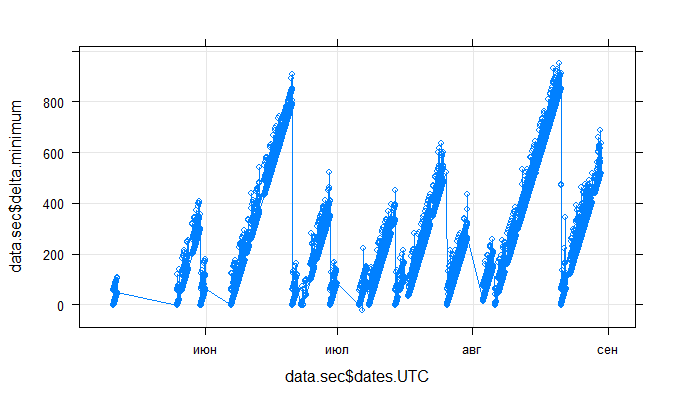
\includegraphics[width=0.9\linewidth]{images/deprontimedifference}
	\caption[Временной ряд разницы приборного времени и меток начала записи в 
	файл.]{Временной ряд разницы приборного времени и меток начала записи в 
		файл. Показаны первые шесть месяцев после запуска спутника Ломоносов, 
		отключения прибора соответствуют циклограмме летных испытаний, а 
		пробелы в данных в начале месяца соответствуют ошибочным номерам дня в 
		месяце.}
	\label{fig:deprontimedifference}
\end{figure}

При привязке секундных данных к баллистическим данным была обнаружена еще одна 
проблема с метками времени в данных 
ДЭПРОН, связанная с постоянным уходом приборных часов. Для решения этой 
проблемы также был разработан алгоритм \ref{list:timecor} и успешно применен 
для восстановления меток времени 

\subsubsection{Описание алгоритма восстановления дат}

На первом этапе  бинарные данные каждого сброса распаковываются в текстовый вид 
с получением таблицы с колонками: \texttt{YYYY-MM-DD hh:mm:ss-1s,	count.h,	
count1,	count2,	count.both,	n1,	n2,	dose1, dose2,	filename,	timestamp}. 
Далее осуществляется разделение текстового поля с меткой времени --- 
\texttt{YYYY-MM-DD hh:mm:ss-1s} на дату и время, а после полученное поле 
\texttt{date} на год, месяц и день - обозначенные \texttt{year, month, day} 
соотвественно.

Создается поле \texttt{dates} имеющее тип данных \texttt{ISOdate} исходя только 
из полей даты года и месяца, а день месяца устанавливается первый. Далее к полю 
\texttt{dates} 
добавляется число дней из поля \texttt{day}, минус один день. В последнюю 
очередь в поле \texttt{dates} выставляется приборное время, отделенное в начале 
алгоритма.

\subsubsection{Описание алгоритма восстановления метки времени}

Приборное время ДЭПРОН установлено на третий часовой пояс и соотвествует 
Московскому 
времени, поэтому для унификации базы данных получено поле \texttt{dates.UTC} 
соответствующее приборному времени смещенному на 3 часа.



Далее в результате ручного анализа данных было найдено что за сутки внутренние 
часы ДЭПРОН уходят вперед на 57 секунд, что хорошо видно на графике~
\ref{fig:deprontimedifference} поэтому был введена поправка \texttt{kt}:
\[ kt = (56.77315002) /86400 \]
Далее c использованием полученной поправки из времени UTC получено 
скорректированное приборное время, хотя это время смещено отностительно 
действительного всемирного времени это смещение меняется каждый раз при 
выключениях прибора в ходе программы исследований \ref{fig:deprontimeplot}. 

\begin{figure}
	\centering
	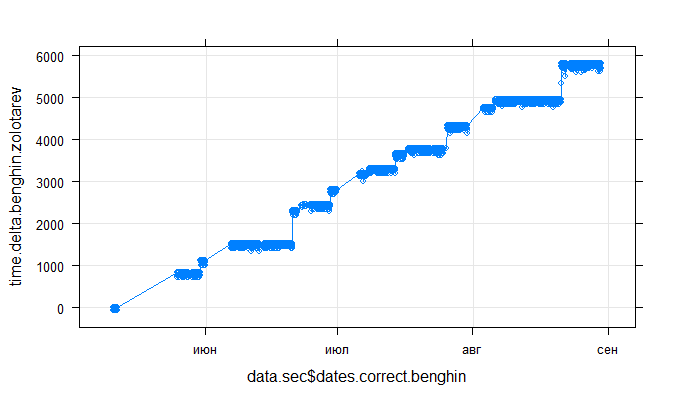
\includegraphics[width=0.9\linewidth]{images/deprontimeplot}
	\caption[Временной ряд разницы калиброванного приборного времени и меток 
	начала записи в файл.]{Временной ряд разницы калиброванного приборного 
	времени и меток начала записи в файл.}
	\label{fig:deprontimeplot}
\end{figure}


Для автоматического определения этого смещения необходимо привязать его к 
независимому источнику точного времени - в качестве такого рассмотрены метки 
времени начала записи в бинарный файл данных БИ а также метки окончания записи 
файловой системы. Оказалось что разница времени меток последней записи сильно 
разнится относительно всех других меток, видимо по причине буферизации записи в 
файл данных, поэтому в качестве реперного времени выбрано время создания файла, 
которое записано в названии каждого файла как POSIXtime в виде 
шестнадцатеричного числа.

После получения разницы ``горизонтального'' приборного времени с временем 
начала записи в файл (поле time.delta.file.start) мы рассчитываем минимум 
(\texttt{delta.minimum}) этой разницы для каждого файла бинарных данных. Анализ 
распределения минимумов показал что моменты ``перескоков'' приборного времени 
из-за выключений приводят к разницам более двух минут, таким образом времена 
выключений были отсеяны от минутных или двухминутных пропусков в при записи в 
бинарных файлах данных. На основе данных о перескоках времени составлен массив 
\texttt{data.sec.switches}, который записывается в отдельный файл и также 
исходный массив секундных данных разбивается на участки без выключений прибора. 

Для каждого участка непрерывной работы были найдены наиболее часто 
встречающиеся значения смещений \texttt{mfv.delta} --- мода разниц. И в 
соответствии с этими значениями скорректировано приборное время.

Последней операцией производится смещение полученного правильного времени на 59 
секунд назад, так как прибор присваивает метку времени массиву данных по окончании периода измерения длительностью 1 минута для массивов А и  5 минут для массивов S. 

Итоговый график сдвигов времени в массивах для одного из дней работы прибора представлен на рисунке \ref{fig:deprontime172}. По оси ординат отложен сдвиг метки времени в блоке данных, длительность которых около 6 минут. Можно заметить что полученные массивы данных после 9:00 начинают иметь пробелы по времени - выпавшие данные измерений длительностью одна минута, эта особенность связана с загруженностью канала приема-передачи, таким образом пробелы в этих данных сказывается на ухудшении по-секундной подробной записи, но поминутная запись данных содержит интегральную информацию по всем счетчикам потоков и дозы.






\begin{figure}
	\centering
	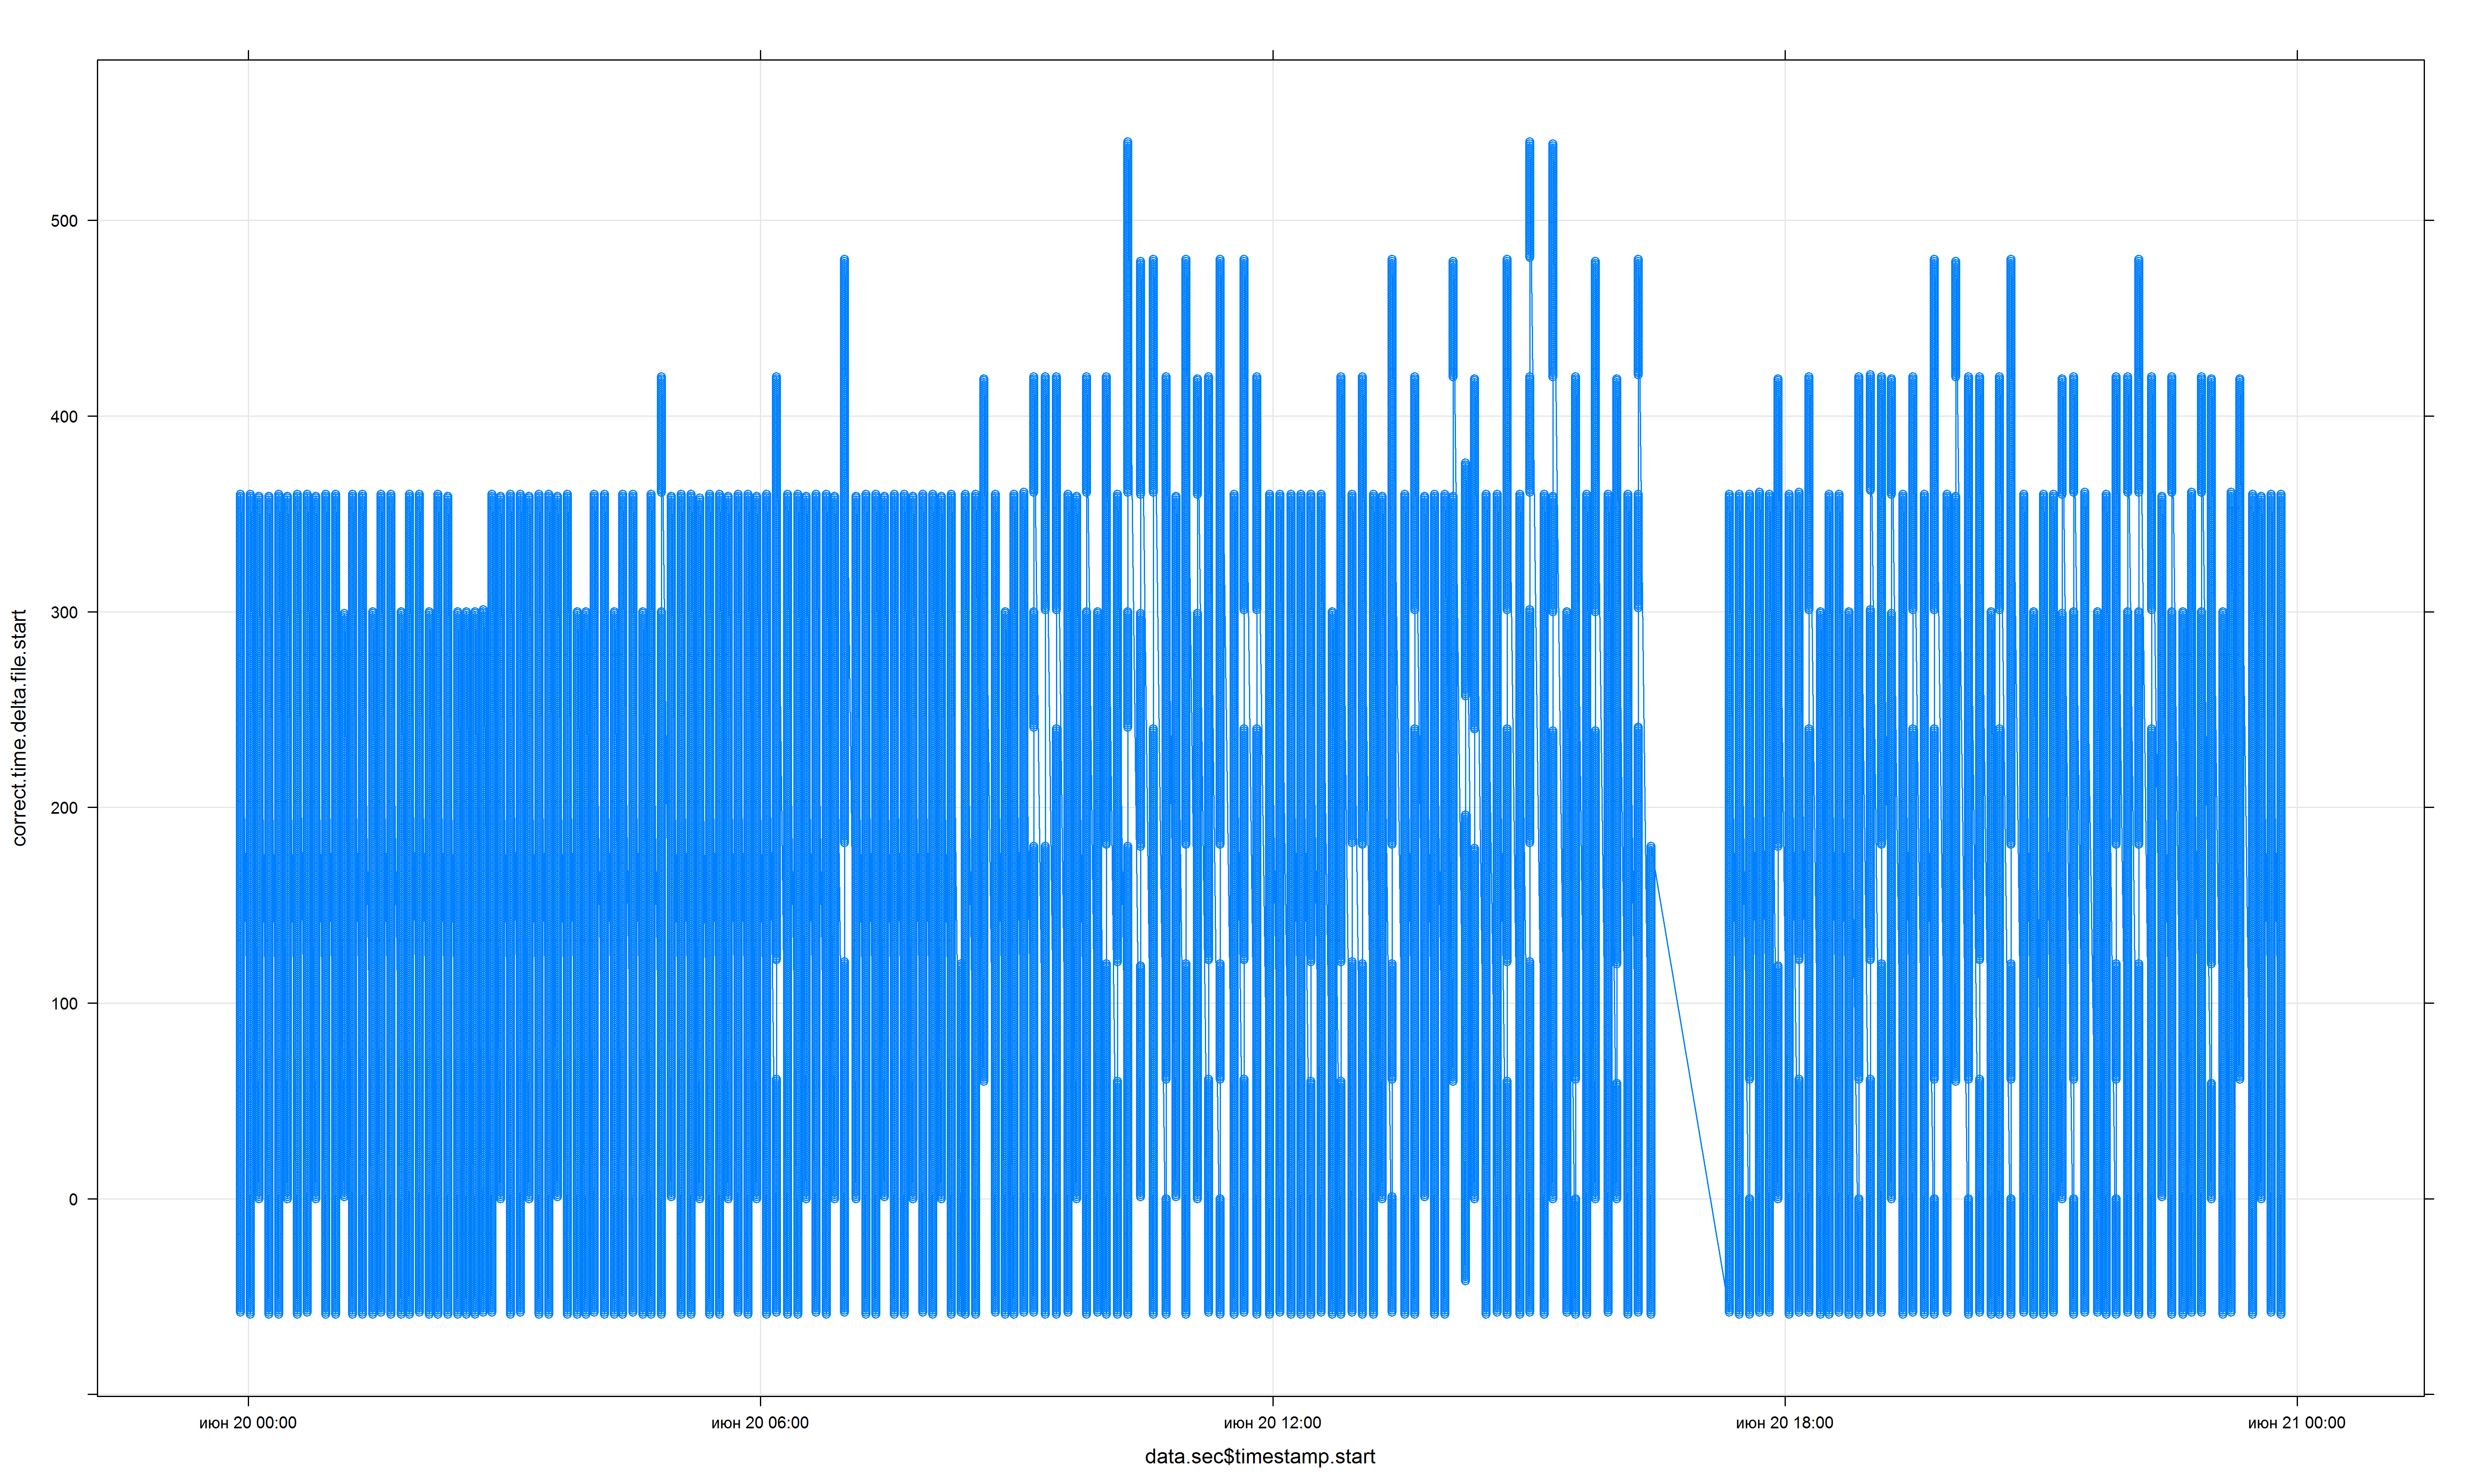
\includegraphics[width=0.9\linewidth]{images/depron_time_172}
	\caption{Пример восстановления меток времени 20 июня 2016 года}
	\label{fig:deprontime172}
\end{figure}






